\documentclass[a4paper,12pt]{article}
\usepackage{amsmath}
\usepackage{graphicx}
\usepackage{datetime2}
\usepackage{url}
\usepackage{amsfonts}
\usepackage{extarrows} 
\usepackage{makecell}
\usepackage{placeins}
\usepackage{fancyhdr}
\usepackage{tikz}
\usepackage{physics}
%\usepackage{mathabx}
\usepackage[]{algorithm2e}
\usepackage[skins]{tcolorbox}
\usepackage{subcaption} 
\usetikzlibrary{positioning,calc}
\usepackage{draftwatermark}
\usepackage{framed}
\SetWatermarkText{DRAFT}
\SetWatermarkScale{5}

\usepackage[left=1in,right=1in,top=1.2in,bottom=1.2in]{geometry}

\newcommand{\tikzmark}[1]{\tikz[overlay,remember picture] \node (#1) [anchor=base] {};}
\newcommand{\snode}[3]{\node [] (#1) at (#2) {$\mathstrut #3$}}
\newcommand{\spath}[2]{\draw[<->] (#1) -- (#2) node [midway, above] () {S}}
\newcommand{\ppath}[2]{\draw[<->] (#1) -- (#2) node [midway, above] () {P}}
 
\fancypagestyle{firstpage}{%
\fancyhf{} % clear all six fields
\renewcommand{\headrulewidth}{0pt}
\renewcommand{\footrulewidth}{0pt}
}
\fancypagestyle{firstcoverpage}{%
\fancyhf{} % clear all six fields
\fancyfoot[C]{\thepage}
\renewcommand{\headrulewidth}{0pt}
\renewcommand{\footrulewidth}{0pt}
}
\fancypagestyle{followingpage}{%
\fancyhf{} % clear all six fields
\fancyhead[LE,RO]{\textbf{\thepage}}
\fancyhead[LO,RE]{\nouppercase{\rightmark}}
\renewcommand{\headrulewidth}{0.7pt}
\renewcommand{\footrulewidth}{0pt}
}
\pagestyle{followingpage}
 

%\documentclass[aip,reprint]{revtex4-1}

\newcommand{\ovl}{\overline}
\newcommand{\unl}{\underline}
\newcommand{\oli}{\overline{i}}
\newcommand{\olj}{\overline{j}}
\newcommand{\olk}{\overline{k}}
\newcommand{\oll}{\overline{l}}
\newcommand{\ola}{\overline{a}}
\newcommand{\olb}{\overline{b}}
\newcommand{\olc}{\overline{c}}
\newcommand{\old}{\overline{d}}

\newcommand{\ooli}{\overline{\overline{i}}}
\newcommand{\oolj}{\overline{\overline{j}}}
\newcommand{\oolk}{\overline{\overline{k}}}
\newcommand{\ooll}{\overline{\overline{l}}}
\newcommand{\oola}{\overline{\overline{a}}}
\newcommand{\oolb}{\overline{\overline{b}}}
\newcommand{\oolc}{\overline{\overline{c}}}
\newcommand{\oold}{\overline{\overline{d}}}

\newcommand{\ool}[1]{\overline{\overline{#1}}}

\newcommand{\eps}{\epsilon}

\newcommand{\olI}{\overline{I}}
\newcommand{\olJ}{\overline{J}}
\newcommand{\olK}{\overline{K}}
\newcommand{\olL}{\overline{L}}
\newcommand{\olA}{\overline{A}}
\newcommand{\olB}{\overline{B}}
\newcommand{\olC}{\overline{C}}
\newcommand{\olD}{\overline{D}}

\newcommand{\doti}{\hat{i}}
\newcommand{\dotj}{\hat{j}}
\newcommand{\dotk}{\hat{k}}
\newcommand{\dotl}{\hat{l}}

\newcommand{\dota}{\hat{a}}
\newcommand{\dotb}{\hat{b}}
\newcommand{\dotc}{\hat{c}}
\newcommand{\dotd}{\hat{d}}

\newcommand{\odota}{\overline{\dota}}
\newcommand{\odotb}{\overline{\dotb}}
\newcommand{\udoti}{\underline{\doti}}
\newcommand{\udotj}{\underline{\dotj}}
\newcommand{\udotk}{\underline{\dotk}}
\newcommand{\odotc}{\overline{\dotc}}

\newcommand{\uli}{\underline{i}}
\newcommand{\ulj}{\underline{j}}
\newcommand{\ulk}{\underline{k}}
\newcommand{\ull}{\underline{l}}
\newcommand{\ulm}{\underline{m}}
\newcommand{\uln}{\underline{n}}

\newcommand{\ulgm}{\underline{\mu}}
\newcommand{\olgm}{\overline{\mu}}
\newcommand{\ulgn}{\underline{\nu}}
\newcommand{\olgn}{\overline{\nu}}
\newcommand{\ulgk}{\underline{\kappa}}
\newcommand{\ulgt}{\underline{\tau}}
\newcommand{\ulgl}{\underline{\lambda}}
\newcommand{\olgl}{\overline{\lambda}} % use for b
\newcommand{\olga}{\overline{\alpha}}
\newcommand{\olgb}{\overline{\beta}}
\newcommand{\olgs}{\overline{\sigma}} % use for a
\newcommand{\olgg}{\overline{\gamma}} 
\newcommand{\olgd}{\overline{\delta}}

\newcommand{\gm}{\mu}
\newcommand{\gn}{\nu}
\newcommand{\gk}{\kappa}
\newcommand{\gl}{\lambda}
\newcommand{\ga}{\alpha}
\newcommand{\gb}{\beta}
\renewcommand{\gg}{\gamma}
\newcommand{\gd}{\delta}
\newcommand{\gs}{\sigma}

\newcommand{\pa}{^{(\alpha)}}
\newcommand{\pt}{^{(\theta)}}
\newcommand{\pdg}{^{\dagger}}
\newcommand{\ptw}{^{(\theta,\omega)}}

\newcommand{\calJ}{\mathcal{J}}
\newcommand{\calK}{\mathcal{K}}
\newcommand{\calZ}{\mathcal{Z}}

\newcommand{\cn}[2]{\left( #1 \mid #2 \right)}
\newcommand{\mbf}[1]{\mathbf{#1}}
\newcommand{\bfun}[2]{\chi_{#1}(\mathbf{r_{#2}})}
\newcommand{\cbra}[1]{\left( #1 \right\rvert }
\newcommand{\cket}[1]{\left\lvert #1 \right)}
\newcommand{\B}[2]{B_{#1}^{#2}}
\newcommand{\x}[2]{_{#1}^{#2}}
\newcommand{\xlr}[1]{\xleftrightarrow{#1}}
\newcommand{\wpa}{\left\lvert w\pa \right\rvert}

\newcommand{\bk}[2]{\bra{#1} \ket{#2}}
\newcommand{\sbk}[2]{\bra{#1} {} \ket{#2}}

\newcommand{\ep}{\epsilon}

\newcommand{\ccpx}[1]{\mathcal{O}(N^{#1})}

\newcommand{\sym}[2]{_{#1 \leftrightarrow #2}}

\newcommand{\ssg}{^{\sigma}}

\newcommand{\mbfx}{\mathbf{x}}

\setcellgapes{10pt}

\newtcolorbox{myframe}[2][]{%
  enhanced,colback=white,colframe=black,coltitle=black,
  sharp corners,boxrule=0.4pt,
  fonttitle=\itshape,
  attach boxed title to bottom right={yshift=0.3\baselineskip+0.4pt,xshift=-2mm},
  boxed title style={tile,size=minimal,left=0.5mm,right=0.5mm,
    colback=white,before upper=\strut},
  title=#2,#1
}

\allowdisplaybreaks 

\newcommand{\forcond}{$\alpha=0$ \KwTo $n_{lap}$}
\newcounter{ISTEP}
\newcommand{\itemR}{\item \refstepcounter{ISTEP}}

\def\signed #1{{\leavevmode\unskip\nobreak\hfil\penalty50\hskip2em
  \hbox{}\nobreak\hfil(#1)%
  \parfillskip=0pt \finalhyphendemerits=0 \endgraf}}

\newsavebox\mybox
\newenvironment{aquote}[1]
  {\savebox\mybox{#1}\begin{quote}}
  {\signed{\usebox\mybox}\end{quote}}

%\newcommand{\nperp}{^{\not\perp}}

\begin{document}

\author{Maximilien Alexandre Ambroise}
\title{My PhD thesis}

\maketitle

This is a fancy front page: contains supervisors, university name, location, exam date ...

\newpage

Licensing

\newpage

(empty)

\newpage

\tableofcontents

\newpage

\section{Introduction}

This is the introduction. Talk about sparsity. Show sparse matrix. How does sparsity arise, what can we do with it, where else does it emerge?
State of arts: adc now, adc in the future

\begin{figure}
\centering
\includegraphics[scale=0.05]{Pics/fock.pdf}
\caption{Adenine-guanine fock matrix Hartree FOck cc-pVTZ}
\label{SparseExample}
\end{figure}

\newpage

\part{Theory: The Basics}

\section{Ground Work}

\subsection{The Schrödinger Equation}

\subsection{Basis Sets}

\subsection{Electron Integrals}

\section{Hartree Fock}

\section{Post-Hartree Fock Ground State}

\subsection{Configuration Interaction}

\subsection{Perturbation Theory}

\subsection{Coupled Cluster}

\section{Post-Hartree Fock Excited State}

\subsection{Configuration Interaction}

\subsection{Coupled Cluster Linear Repsonse}

\subsection{Equation-of-Motion Coupled Cluster}

\subsection{Algebraic Diagrammatic Construction}

\section{Density Fitting}

\part{Theory: Reduced-Cost QC}

While computational chemistry has manifested itself as a popular and widely used tool, its inherently steep scaling limits its applicibality to cheaper methods like DFT, orto small or middle sized molecules for post-Hartree Fock methods. Even Hartree Fock with O(N$^3$) expensive when comparing to the rest of the world of computer science (examples?). Very early on, with the development of CI methods, (Pulay) effort has been put into reducing the prefactor and computational complexity for QC methods. Example: One of the most time-consuming steps in Post-Hartree Fock is the formation of the molecular orbitals, e.g. formation of the OVOV block of the MO integral tensor as encountered in CC and MP2:
\begin{equation}
\cn{ia}{jb} = \sum^{vir}_b C_{\sigma b} \sum^{vir}_a C_{\nu a} \sum^{occ}_j C_{\lambda j} \sum^{occ}_i C_{\mu i} \cn{\mu\nu}{\lambda\sigma}
\end{equation}
By efficiently refactoring the sums, the MO-AO integral transformation scales as O(N$^4$). There are two reasons for the large cost: first, and quite obviously, a rank-4 tensor scales very fast, hence O(N4), also becomes a bottle neck for tensor contractions as many indices. Secondly, for large basis sets with triple-zeta quality or higher, or basis sets with diffuse functions, the virtual orbital space is very large, and can be multiple times the size of the occupied space. 
Attempts to reduce scaling can be grouped into two groups: screening-based methods and domain-based methods. Screening-based methods recast existing equations into the AO basis and use the sparsity and fast decay between AOs to establish highly efficient screening algorithms to lower the scaling of integral transformation. Domain-based methods stay in the MO basis, but a localized one, and attempt to assign domains of virtual molecular orbitals to a single LMO or a pair of LMOs, to obtain a more compact representation. 
Other attempts at mitigating the cost of MO-AO transformation is to exploit the rank sparsity of the AO ERI tensor. Density fitting and Cholesky decompositions can refactor the ERI tensor into a product of two 3-dim tensors. Tensor Hypercontraction goes even further and decomposes into 4 2-dim tensor. Density does not inherently lower scaling of methods, but rather reduces the prefactor associated with integral transformation. In special cases, decomposition techniques allow a refactoring of the working equations into lower scaling. Examples include the coulomb part of the Fock-build (O3 to O2) and SOS-MP2, SOS-CC2 or SOS-ADC(2) (O5 to O4).  
Density fitting and local approximations can be combined, to yield the best of both world in what is known as local density fitting.
All of the above methods have their fair share of problems, some more than others. We will first address principles of density fitting, before looking at possible orbital representations, and how they can be used for reduced scaling. Also go to local density fitting, and finally how the methods are implemented for ground state (HF,MP2,CCSD) and excited state computations (CI, CCLR, ADC).

\section{Density Fitting}
About density fitting. Principles

\section{Sparsity in Electronic Structure Theory}

Sparsity is a core concept in electronic structure theory. Many of the most commonly encountered matrices and tensors exhibit some form of sparsity. 

\FloatBarrier

\subsection{Scaling of Electron Integrals}

Molecular electron integral evaluation can become prohibitively expensive for large systems, espcially the four-dimensional ERI tensor which formerly scales as $\ccpx{4}$. It is therfore imperative to exploit the exponential decay of the GTO basis.

Consider a model system consisting of $n$ hydrogen atoms arranged in a line, with a distance of 1 $a_0$ between one another, and a primitive 1s Gaussian function attached to each atom. Figure ... shows the scaling behaviour for the overlap and electron repulsion integrals of this system. A full line is used to show the number of total elements, while the dotted line represents the number of significant integrals with magitude $>$ 1e-10. From observing both graphs, it becomes apparent that for increasing number of atoms, many of the electron integrals can be ignored. 

\subsubsection{Linear Scaling Overlap Integrals}

While the overlap integrals formely scale with $\ccpx{2}$, it can be shown that the number of significant elements scales \emph{linearly}. First, consider the product of two 1s GTOSs $\chi_{A}$ and $\chi_{B}$, centred at $\mathbf{A}$ and $\mathbf{B}$, with exponents $\alpha$ and $\beta$. The Gaussian product theorem (GPT) states that the result is itself also a (scaled) Gaussian function
\begin{equation}
\chi(A,\alpha) \chi(B,\beta) = e^{-\alpha \left\lvert \mathbf{r} - \mathbf{A} \right\rvert^2} e^{-\beta \left\lvert \mathbf{r} - \mathbf{B} \right\rvert^2} = \kappa \chi(P,\alpha+\beta)  
\end{equation}
\noindent with the scaling factor $\kappa$ 
\begin{equation}
\kappa = e^{-\frac{\alpha\beta}{\alpha+\beta}\left\lvert \mathbf{A} - \mathbf{B} \right\rvert^2}
\end{equation}
\noindent and the centre-of-charge coordinate $P$
\begin{equation}
\mathbf{P} = \frac{\alpha \mathbf{A} + \beta \mathbf{B}}{\alpha + \beta}
\end{equation}
\noindent Spatioal integration yields the expression for the overlap between $\chi_A$ and $\chi_B$
\begin{equation}
S_{AB} = \int \kappa \chi_{P} dr = \kappa \left(\frac{\pi}{\alpha + \beta}\right)^{3/2}
\end{equation} 
\noindent The magnitude of the overlap integral is proportional to the scaling factor $\kappa$ which decays exponentially with the distance between GTO centres. In the case of the model system given above, where $\alpha = \beta$, the distance at which the integral falls below a certain threshold $\eps$ is given by 
\begin{equation}
d_s = \sqrt{\alpha^{-1} ln \left[ \left( \frac{\pi}{2\alpha}\right)^3 \eps^{-1/2} \right]}
\end{equation} 
\noindent Which in our case is equal to 6.9 $a_0$. Each hydrogen atom therefore only has significant overlap with a finite number $n_{max}$ of other centres. For atom chains with $n > n_{max}$, the number of non-zero elements in the overlap matrix will no longer scale as $n^2$, but \emph{linearly} with $nn_{max}$. For more realistic, three-dimnensional molecular systems, the crossover is less clearly defined due to the non-uniform distribution of atoms and different GTO exponents. Nonetheless, if a system grows sufficiently large, the overlap integrals still scale linearly. Similar arguments can be brought forth for the kinetic-energy integrals as well. 

\subsubsection{Quadratic Scaling Electron Repulsion Integrals} 

Using the Guassian product theorem established above, we can express the two-electron repulsion integrals of four primtive 1s Gaussian functions $s(A,\alpha)$, $s(B,\beta)$, $s(C,\gamma)$ and $s(D,\delta)$ as
\begin{equation}
\begin{split}
g_{ABCD} &= \int s(A,\alpha) s(B,\beta) \frac{1}{\left\lvert \mathbf{r_1} - \mathbf{r_2} \right\rvert} s(C,\gamma) s(D,\delta) dr \\
&= \int \kappa s(P, \alpha+\beta) \frac{1}{\left\lvert \mathbf{r_1} - \mathbf{r_2} \right\rvert} \lambda s(Q, \gamma+\delta)
\end{split}
\end{equation}
\noindent where $s(P,p)$ and $s(Q,q)$ are Gaussian distributions with
\begin{equation}
\mathbf{P} = \frac{\alpha \mathbf{A} + \beta \mathbf{B}}{\alpha + \beta} ; \quad \mathbf{Q} = \frac{\gamma \mathbf{C} + \delta \mathbf{D}}{\gamma + \delta}
\end{equation}
\begin{equation}
\kappa = e^{-p\left\lvert \mathbf{A} - \mathbf{B} \right\rvert^2} ; \quad \lambda = e^{-q\left\lvert \mathbf{C} - \mathbf{D} \right\rvert^2}
\end{equation}
\begin{equation}
p = \frac{\alpha\beta}{\alpha+\beta}; \quad q = \frac{\gamma\delta}{\gamma+\delta}
\end{equation}

\noindent The coulomb integrals can then be evaluated as 
\begin{equation}
g_{ABCD} = \sqrt{\frac{4 \eta}{\pi}} S_{AB} S_{CD} F_0\left(\eta \left\lvert \mathbf{P} - \mathbf{Q} \right\rvert^2 \right)
\end{equation}
\noindent with the Boys function $F_0$ and the reduced exponent $\eta$ given by
\begin{equation}
\eta = \frac{pq}{p+q}
\end{equation}

\noindent The Boys function is an important function appearing in many expressions for molecular integral evaluation. There are two expressions that bound the Boys function
\begin{equation}
\begin{split}
F_n(x) \leq \frac{1}{2n+1} \quad \textrm{for small } x \\
F_n(x) \leq \frac{(2n-1)!!}{2^{n+1}}\sqrt{\frac{\pi}{x^{2n+1}}} \quad \textrm{for large } x 
\end{split}
\end{equation}
\noindent Using the Boys function's upper bounds, we can derive an upper bound for the electron repulsion integrals of our model system
\begin{equation}
g_{ABCD} \leq min \left\lbrace \sqrt{\frac{4\eta}{\pi}} S_{AB} S_{CD}, \frac{S_{AB} S_{CD}}{\left\lvert \mathbf{P} - \mathbf{Q} \right\rvert} \right\rbrace
\end{equation}
\noindent The left-hand upperbound represents the short-range limit of the Boys function, and the right-hand one the long-range limit. In the short-range limit, i.e. for increasing distance $R_{AB}$ or $R_{CD}$, the magnitude of $g$ decreases exponentially. As shown in the previous section, the non-zero elements of the overlap integrals $S_{AB}$ and $S_{CD}$ scale linearly with system size, and therefore the number of significant electron repulsion integrals scales with $N^2$ in total. 
It should be noted, that in the long-range limit whith increasing distance $R_{PQ}$ between product densities, the elements in $g$ will eventually scale linearly. However, the $1/R$ decay of the long-range interactions is so slow that it becomes practically useless. In the case of the hydrogen atom chain, the integrals $\cn{\mu\mu}{\nu\nu}$ only fall below 1e-10 for $R_{PQ}$ greater than 10$^{10}$ $a_0$. While the long-range decay is impractical for use in the case of the electron repulsion integrals, there are instances such as in AO-MP2 where the \emph{bra} and \emph{ket} decay as $1/R^4$. 

\begin{figure}
\begin{minipage}{0.5\linewidth}
\includegraphics[scale=0.7]{overlap_nze}
\caption{Number of significant ...}
\end{minipage}
\begin{minipage}{0.5\linewidth}
\includegraphics[scale=0.7]{eri_nze}
\caption{Number of significant ...}
\end{minipage}%
\end{figure}

\begin{figure}
\begin{minipage}{0.5\linewidth}
\includegraphics[scale=0.7]{overlap_decay}
\caption{Number of significant ...}
\end{minipage}
\begin{minipage}{0.5\linewidth}
\includegraphics[scale=0.7]{eri_decay}
\caption{Number of significant ...}
\end{minipage}%
\end{figure}

Most of the frustrations stem from N$^2$ AO ERI, but N$^4$ MO ERI
Show a graph of AO ERI of H2: (mn,mn) vs (mm,nn)
% Good explanation for "linked indices rule" https://aip.scitation.org/doi/pdf/10.1063/1.4926879

\FloatBarrier

\section{The ABCs of LMOs: Orbital Representations}

A small intro

%\url{https://link.springer.com/article/10.1007/s00894-018-3880-8}

Occupied and virtual molcular orbitals can generally be represented in two ways: canonical molecular orbitals (CMOs) and local molecular orbitals (LMOs). CMOs are the eigenvectors of the Fock matrix obtained by solving the eigenvalue problem

\begin{equation}
\mathbf{F}\mathbf{C} = \mathbf{S}\mathbf{C} \eps
\end{equation}

where the eigevalues $\epsilon$ are known as the molecular orbital energies of the associated CMOs. However, CMOs are not unique in the sense that there are multiple molecular representations possible which yield the same electron density $\mathbf{P}$. Observables such as the electron density, or the total energy, are said to be invariant under unitary transformations (Fock V (1930) Z Phys 61:26–148). The CMOs $\mathbf{C}$ relate to other representations $\mathbf{L}$ as

\begin{equation}
L_{\mu \uli} = U_{\uli i} C_{\mu i}
\end{equation}

\noindent where $\mathbf{U}$ is a unitary transformation matrix with $\mathbf{U}^{\dagger} \mathbf{U}$ = $\mathbb{1}$. Typically, $\mathbf{U}$ is chosen to generate a set of molecular orbitals which are localized on as few atoms as possible, hence local molecular orbitals. While CMOs and LMOs agree on observables, they show differences for non-obervables, such as molecular orbital energy or orbital shape.

There are several reasons for choosing an LMO representation. First, as mentioned above, LMOs are used in local correlation methods, because CMOs are too delocalized, and electron correlation between LMO centres decay more rapidly. Secondly, they offer a more intuitive picture for chemists and help to interpret chemical phenomena (cite), e.g. invloving lone pairs or $\pi$ bonds. Different representations can be used to interpret different phenomena, e.g. Boys LMOs vs NTOs.

Over the years, a myriad of different schemes has been proposed on how to find appropriate tranformation matrices $\mathbf{U}$. We will now go over some examples.

\subsection{Local Molecular Orbitals}

Some words about it

\subsection{LMOs by Reducing a Functional}
% (0) https://aip.scitation.org/doi/full/10.1063/1.2360264
% (1) https://journals.aps.org/rmp/abstract/10.1103/RevModPhys.32.296
% (2) https://journals.aps.org/rmp/abstract/10.1103/RevModPhys.35.457
% (3) https://aip.scitation.org/doi/10.1063/1.456588
% (4) J. E. Subotnik, Y. Shao, W. Z. Liang, and M. Head-Gordon, J. Chem. Phys. https://doi.org/10.1063/1.1790971 121, 9220 (2004).
% (5) https://aip.scitation.org/doi/10.1063/1.2033687

One of the most popular methods for finding LMOs consists in maximizing a localization function $\eta(\phi)$ by successive rotation of the orbital space. The most prominent examples are Foster-Boys (FB)(1), Edmiston-Ruedenberg (ER) (2) and Pipek-Mezey (PM) (3). Their functionals can be written as

\begin{eqnarray}
\zeta_{FB}(\chi) = \sum_i \bra{\chi_i} \mathbf{r} \ket{\chi i}^2 \\
\zeta_{ER}(\chi) = \sum_i \cn{\chi_i \chi_i}{\chi_i \chi_i} \\
\zeta_{FB}(\chi) = \sum_i \sum_A \bra{\chi_i} \mathbf{P}_A \ket{\chi i}^2 
\end{eqnarray}

The problem is generally solved using an iterative procedure consisting in consecutive pair-wise rotations, known as Jacobi sweeps (ALGO). These sweeps are rotated until convergence is reached, which may be slow. The methods differ within the procedure by how the rotational angle is computed, and scale diiferently with system size, with $\ccpx{3}$ for FB, $\ccpx{5}$ for ER and $\ccpx{4}$ for PM. A faster alternative to Jacobi sweeps does also exist (4). 

Over the years, PM has been the more popular choice of the three: like ER and unlike FB, it conserves $\sigma$-$\pi$ separation (0),  but it scales more favorably than ER.

Functional localization methods are most often used for rotating occupied MOs. Virtual MOs are often plagued by convergence issues and have a steep computational cost simply due to being much more numerous than occupied MOs (5). It is crucial that molecular localization should not take longer than the methods they are used for, and hence VMOs are often localized using separate methods.

EXAMPLES!! Ethylene

\subsection{Projected Atomic Orbitals}
% (0) https://www.annualreviews.org/doi/10.1146/annurev.pc.44.100193.001241
% (1) https://aip.scitation.org/doi/full/10.1063/1.2173249

A set of highly localized molecular orbitals can be obtained by projecting the CMOs onto the atomic orbital basis, known as projected atomic orbitals (PAO) (0). For a set of orthonormal occupied/virtual molecular orbitals $\{\Psi_i\}$ and $\{\Psi_a\}$, the projection operators are defined as (1)

\begin{eqnarray}
\hat{P} &= \ket{\Psi_i} \bra{\Psi_i} &= \ket{\chi_{\mu}} C_{\mu i} C_{\nu i} \bra{\chi_{\nu}} \\
\hat{Q} &= \ket{\Psi_a} \bra{\Psi_a} &= \ket{\chi_{\mu}} C_{\mu a} C_{\nu a} \bra{\chi_{\nu}}
\end{eqnarray}

The projection operators are idempotent and mutually orthogonal with $\hat{P}\hat{Q} = \mathbb{1}$. Applying the projection operators to the set of AOs 

\begin{eqnarray}
\hat{P} \ket{\chi_{\mu'}} &= \sum_{\mu} \ket{\chi_{\mu}} P_{\mu\nu} S_{\nu\mu'} &= L_{\mu I} \ket{\chi_{\mu}} \\
\hat{Q} \ket{\chi_{\mu'}} &= \sum_{\mu} \ket{\chi_{\mu}} Q_{\mu\nu} S_{\nu\mu'} &= L_{\mu A} \ket{\chi_{\mu}}
\end{eqnarray} 

\noindent yields the set of occipied and virtual PAOs $\{\chi_I\},\{\chi_A\}$. Both sets span a space of $n_{AO}$ functions each, as opposed to $n_{occ}$ and $n_{vir}$. As such, just like the AO basis, the PAO basis is redundant. CMOs are transformed to PAOs by the relationship

\begin{eqnarray}
\ket{\chi_I} = (\mathbf{SC})_{Ii} \ket{\Psi_i} \\
\ket{\chi_A} = (\mathbf{SC})_{Aa} \ket{\Psi_a}
\end{eqnarray}

PAOs are centred on the atom on which their corresponding AO is localized. However, PAOs can still span multiple atoms. Methods which are entirely formulated in PAOs are rare (1).

PAOs also arise in the context of AO-MP2, when rearranging the canoncial equations into an AO basis, as will be shown later.

\subsection{Subspace Projected Atomic Orbitals}

Some applications need localized molecular orbitals that only span a certain region of a molecule, e.g. density matrix embedding theory (DMET) (refs) or local ADC (ref). The molecule is split into two subunits, and atoms are grouped into an active region $A$ and an inactive region $B$ according to specific selection criteria. Region $A$ contains the molecular subunit of interest. 

Most implementations use the Mulliken gross charges to find
... ? Not used for virtuals? Put it into AO-ADC Part?

% SPADES: Cla https://www.osti.gov/pages/servlets/purl/1631165
% SPADES: Cla2019 https://pubs.acs.org/doi/10.1021/acs.jctc.8b01112

\subsection{Cholesky Molecular Orbitals}

Sparsity of the atomic density matrix is crucial for achieving low-scaling electronic structure methods. Aquilante et al. proposed (0) to define a set of occupied molecular orbitals by Cholesky decomposition of the density matrix. Analysis of the resulting Cholesky molecular orbitals (CholMOs) showed their localized character inherited from the sparsity of the density matrix.

\begin{equation}
\mathbf{P} = \mathbf{LL^T}
\end{equation}

Figure ... shows the sparsity of the occupied density matrix and the occupied cholesky molecular coefficient matrix of the linear alkane H$_{322}$C$_{160}$. The number of CholMOs is equal to the rank of the density matrix, which is equal to the number of occupied orbitals. The CholMOs are computed by an incomplete Cholesky decomposition with full row and column pivoting  (ALGO). The unitary transformation matrix is given by

\begin{equation}
U_{i\uli} = C_{\mu i} S_{\mu \nu} L_{\nu \uli}
\end{equation}

The decomposition algorithm scales with $\ccpx{3}$ but can be made linearly scaling by using sparse matrix algebra. CholMOs have several advantages: the Cholesky decomposition is fast and non-iterative, and an initial guess for molecular orbitals is not needed. 

The scheme can be extended to virtual orbitals as well, by CD of the virtual atomic density matrix $\mathbf{Q}$. The rank of $\mathbf{Q}$ is equal to the number of virtual orbitals $n_vir$, therefore the prefactor of the incomplete CD increases with basis set size. Especially in the presence of diffuse functions, the rank reduction might not offer much of an advantage compared to simpler localization methods such as PAOs.  

Moreover, orbitals obtained by CD are less localized than FB or ER LMOs, especially for small molecules. Low scaling is still possible using CholMOs in the context of LMO correlation methods, albeit with a larger prefactor.

CD is also used in the context of AO-MP2 to reduce the prefactor of inetgral transformation by using the rank sparsity of the pseudo-density matrices, as will be shown further below.

CholMOs can also used as an initial guess for iterative localization schemes to achive faster convergence.  

\subsection{Natural Orbitals}

While the schemes described above try to generate a set of occupied and/or virtual molecular orbitals localized in space, natural orbital (NOs) methods try to generate a set of "compact" orbitals, i.e. a minimal set of orbitals that can describe the problem at hand. The concept of natural orbitals was first introduced by Löwdin (A). The natural orbitals $\Theta_i$ of a wave function $\Psi$ are defined as the eigenfunctions of the one-particle density operator $\hat{n}$

\begin{equation}
\hat{n}\ket{\Theta_i} = n_i \ket{\Theta_i} 
\end{equation}

\noindent where $n_i$ are the occupation numbers of the associated orbital $\Theta_i$. One can then choose a reduced orbital space $\{\tilde{\Psi}_i\}$ by only taking into account those orbitals with an occupation number above a certain threshold $\tau$. The orbitals are "natural" in the sense that they are determined purely using $\Psi$, and are intrinsic to the system. NOs are computed by diagonalizing the one-particle density matrix at the desired level of theory (Hartree-Fock, MP, CIS, CC). 

NOs are state-specific (Pok2019), meaning that NOs computed from the ground state densities may not be well suited to describe excited states, and NOs of different excited states might also greatly differ. As such, as will be later shown for local flavours of ADC, NOs need to be recomputed for each state.

% CIS(D) density matrices https://aip.scitation.org/doi/pdf/10.1063/1.4983277

\subsubsection*{Natural Orbitals in Hartree Fock Theory}

In Hartree Fock theory, natural orbitals are mostly reserved for qualitative population and bond order analysis. 

Natural atomic orbitals (NAOs) are computed by diagonalizing the blocks $P_{\mu_A\nu_A}$ of the atomic density matrix, where ${\mu_A}$, ${\nu_A}$ are basis functions centred on atom $A$. NAOs are optimal for describing the electron density around individual atom centres (IUPAC). NAOs are also useful for obtaining a set of guess orbitals from densitiy matrices formed from the superposition of atomic densities (SAD) guess. 

NHOs obtained from NAOs + off-diag NAOs 
% (ref: https://pubs.acs.org/doi/pdf/10.1021/ja00544a007)

NBOs obtained from NHOs

% NBOs https://aip.scitation.org/doi/pdf/10.1063/1.445134

% NAOs, NBOs https://pubs.rsc.org/en/content/articlepdf/2001/rp/b1rp90011k

% (Recent) NBOs https://onlinelibrary.wiley.com/doi/epdf/10.1002/wcms.51

% https://goldbook.iupac.org/terms/view/NT07076

\subsubsection*{Frozen Natural Orbitals}

For large basis sets, CMOs are much more compact than the virtual orbital span, and the number of occupied NOs is not significantly lower than that of occupied CMOs. It is therefore sufficient to only compute the eigenfunctions of the virtual-virtual block of the one-particle density matrix, which are known as frozen natural orbitals (FNOs) (Bar1970). FNOs need information of the correlated wave function, and are therefore typically computed at a lower level of theory. For example, the easiest way to obtain a set of FNOs for CCSD or CCSD(T) computation is to diagonalize the virtual-virtual block  of the MP2 density matrix (Sos1989, Tau2005, Tau2008)
\begin{equation}
D_{ab} = \frac{1}{2} sum_{cij} \frac{K_{ij}^{cb} K_{ij}^{ca}}{\eps_{ij}^{ab} \eps_{ij}^{ca}}
\end{equation}
\noindent with
\begin{equation}
K_{ij}^{ab} = 2 \cn{ia}{jb} - \cn{ib}{ja}
\end{equation}
\begin{equation}
\eps_{ij}^{ab} = \eps_i + \eps_j - \eps_a - \eps_b 
\end{equation}
The FNOs are then canonicalized (see ...). The combined set of occupied CMOs and virtual FNOs forms a very compact representation suitable for CC ground state and excited state calculations.

% MP2 NOs:
% Jor1988 J. Chem. Phys. 88, 3834 (1988); https://doi.org/10.1063/1.453884
% D. M. Silver and R. J. Bartlett,Phys. Rev. A13,1 1976.
% D. M. Silver, S. Wilson, and R. J. Bartlett,Phys. Rev. A16,477 1977.

% FNOs: 
% Bar1970 Phys. Rev. A 1, 644 – Published 1 March 1970

% FNO CC: 
% Sos1989 https://doi.org/10.1016/0009-2614(89)87399-3
% Tau2005 Taube, Andrew G.; Bartlett, Rodney J. (2005). Frozen Natural Orbitals: Systematic Basis Set Truncation for Coupled-Cluster Theory. Collection of Czechoslovak Chemical Communications, 70(6), 837–850. doi:10.1135/cccc20050837  
% A. G. Taube and R. J. Bartlett,  Frozen natural orbital coupled-cluster theory:  Forces andapplication to decomposition of nitroethane,  J. Chem. Phys.128, 164101 (2008)
% CCLR NO  A. Kumar and T. D. Crawford,   Frozen virtual natural orbitals for coupled-cluster linear-response theory,  J. Phys. Chem. A121, 708 (2017).

% Have a look at Pok2019 https://chemrxiv.org/articles/preprint/Extension_of_Frozen_Natural_Orbital_Approximation_to_Open-Shell_References_Theory_Implementation_and_Application_to_Single-Molecule_Magnets/10308053/1

\subsubsection*{Natural Transition Orbitals}

Consider the CIS eigenvalue problem for finding the excitation energies $\omega_n$ and their associated transition density matrices $R_n$

\begin{equation}
\mathbf{A_{CIS}} R_n = \omega_n R_n 
\end{equation}

The matrices $\mathbf{R}_n$ contain $n_{occ}n_{vir}$ expansion coefficients $c_{ia}$ which show how much an orbital-virtual MO pair $ia$ contributes to the excitation $n$. The numer of non-negligebale coefficients can be far from zero, making interpretations of the computed results difficult for some systems.

Natural transition orbitals (NTOs) were introduced to facilitate the qualititative description of an excited state and finding connections to experimental spectra (Luz1976, Mar2003, Mar2008). NTOs are typically obtained by computing the singular value decomposition (SVD) of the state densities $\mathbf{R}_n$

\begin{equation}
\mathbf{R} = \mathbf{U} \mathbf{\Sigma} \mathbf{V}^{\dagger}  
\end{equation} 

\noindent where $\mathbf{U}$ and $\mathbf{V}$ are unitary matrices with dimension $n_{occ} n_{NTO}$ and $n_{vir}n_{NTO}$, and $\Sigma$ is a $n_{NTO}$ by $n_{NTO}$ matrix containg the singular values $s$ on its diagonal. The CMOs $\{\Psi^{occ}_i,\Psi^{vir}_a\}$ are transformed to the NTO basis $\{\overline{\Psi}^{occ}_k,\overline{\Psi}^{vir}_k\}$ using

\begin{equation}
\ket{\overline{\Psi}^{occ}_k} = U_{ki} \ket{\Psi^{occ}_i}
\end{equation}
\begin{equation}
\ket{\overline{\Psi}^{vir}_k} = V_{ka} \ket{\Psi^{vir}_a}
\end{equation}

\noindent The singular value $s_k$ show the contribution of an NTO pair $k$ to the excited state. In most cases, the number of significant NTO pairs is significantly lower than $n_{occ}n_{vir}$ and at most equal to $n_{occ}$. NTOs are not limited to CIS, but can also be obtained by SVD decomposition of the singles-singles block of excited state densities from higher order methods such as ADC or CCLR. 

Natural transition orbitals have also found use in local excited  state correlation methods (Bau2017,Hof2017), where CIS NTOs are combined with MP2 NOs to obtain a compact orbital representation for ground and excited state coupled cluster calculations.

EXAMPLE!!! phenylalanine

% Luz1976 https://link.springer.com/article/10.1007%2FBF00526670

% Mar2003 https://aip.scitation.org/doi/pdf/10.1063/1.1558471

% https://www.sciencedirect.com/science/article/pii/S0009261407002072?via%3Dihub

% CornFlex: Bau2017 https://aip.scitation.org/doi/pdf/10.1063/1.4984820

% Hof2017 Natural transition orbitals for the calculation of correlation andexcitation energies


\subsection{Specific Virtual Orbitals}

In most cases, using LMOs instead of CMOs does not offer any a priori advantage in terms of the computational complexity asscociated with correlated methods, and additional apprximations are necessary. In LMO correlation methods, this is often done by truncating the VMO space. TRuncation of the VMOs has been an active field of research for "a long time", and several schemes have emerged over the years. A naive approach to truncate the virtual space would be to eliminate VMOs with orbital energies above a certain threshold; however, this proved to be unusable in most contexts (ref). More successful methods for VMO truncation use the concept of what we will refer to as \emph{specific virtual orbitals} (SVOs). SVOs are specific in the sense that each individual LMO $i$ or each pair of LMOs $ij$ has their own set of SVOs $a_i$ (orbital specific virtual orbitals) or a$_{ij}$ (pair specific virtual orbitals) associated to it.
The concept of SVOs naturally arises in the context of correlated methods such as the coupled electron pair approximation (CEPA) where the total energy is computed is computed as the sum of electron pair energies $e$
\begin{equation}
E_{CEPA} = \sum_{ij} e_{ij}
\end{equation}
The electron pair energy decays rapidly as a function of the distance $r$ between MO centres in an LMO basis. Distant virtual orbitals contribute less to the elctron pair energy as virtual orbitals close to ${ij}$. It has been shown early on that instead of using the whole virtual orbital span, one can correlate only a subset or reduced set of virtual orbitals with each electron pair (0,1,2,3) and still recover most of the correlation energy. In the limit of large molecules, the number of signiciant virtual orbitals for an electron pair becomes independent of system size (4). There are different ways to choose how to define the VMO subsets.

Include this: Pair apprximations Electron pairs are first grouped by distance $r$ between occuied LMOs: strong pairs ($1 < r \leq 8 a_0$), weak pairs ($8 < r \leq 15 a_0$) and very distant pairs ($15 < r$).
Very distant: lower level of theory, or neglected Talk about how they are transformed? (4)

% 0 BASIS FOR LMO-PAO S. Saebø and P. Pulay , Chem. Phys. Lett., 1985, 113 , 13
% 1 BASIS FOR PNOs Edmiston, C.; Krauss, M. Configuration-interaction calculation of H3 and H2. J. Chem. Phys. 1965, 42, 1119– 1120,  DOI: 10.1063/1.1696050 
% 2 OTHER Meyer, W. Ionization energies of water from PNO-CI calculations. Int. J. Quantum Chem. 1971, 5, 341– 348,  DOI: 10.1002/qua.560050839 
% 3 ALSO Meyer, W. PNO-CI Studies of electron correlation effects. I. Configuration expansion by means of nonorthogonal orbitals, and application to the ground state and ionized states of methane. J. Chem. Phys. 1973, 58, 1017– 1035,  DOI: 10.1063/1.1679283
% 4 https://pubs.rsc.org/am/content/articlehtml/2012/cp/c2cp40231a#cit51

\subsubsection*{Domain Specific Virtual Orbitals}

We call domain specific virtual orbitals (DSVOs) any type of virtual orbitals where the subsets are formed \emph{a priori} by distance criteria. Examples include the local MP2 and local CCSD implementations by Schütz et al.(AA,AB,AC)

First, occupied CMOs are localized by one of the methods described above. The method of choice in Ref [AA-AC] was the Foster-Boys scheme. Virtual CMOs are recast into the PAO basis. Each individual occuied LMO $\ket{\Psi_i}$ is then assigned a subset $[i]$ of PAOs, chosen by a Boughton-Pulay (BP) criterium (AD) or by population analysis (AE). 

For a given electron pair $ij$, the pair domain is then formed by taking the union $[ij]$ = $[i] \bigcup [j]$. The set of all virtual pair domains $[ij]$ forms the DSVOs.

Alongside AOs, DSVOs were among the first orbital representations in which linear scaling correlated methods were formulated. Their dependency on distance criteria for selecting the pair domains makes them less rigorous than other methods. 

% Local LMO-PAO
% AA M. Schütz , G. Hetzer and H.-J. Werner , J. Chem. Phys., 1999, 111 , 5691
% AB M. Schütz and H.-J. Werner , J. Chem. Phys., 2001, 114 , 661
% AC M. Schütz and H.-J. Werner , Chem. Phys. Lett., 2000, 318 , 370 
% AD https://onlinelibrary.wiley.com/doi/abs/10.1002/jcc.540140615
% AE R. A. Mata, H.-J. Werner, S. Thiel and W. Thiel, J. Chem. Phys., 2008, 128, 025104

\subsubsection*{Pair Natural Orbitals}
% Review: https://pubs.rsc.org/am/content/articlehtml/2012/cp/c2cp40231a
First introduced under the guise of "pseudo-natural orbitals" (Edmiston), then rediscovered by Neese (CA,CB,CC), projected natural orbitals (PNOs) have risen in popularity in the recent years (refs). Similarly to DSVMOs, each electron pair has a set of PNOs associated to it. PNOs are formed by diagonalizing the MP2 pair density matrix for each LMO pair $ij$

\begin{equation}
\mathbf{D}^{ij} = \frac{1}{1+\delta_{ij}} \left(\tilde{\mathbf{t}}^{ij} \mathbf{t}^{ij} + tilde{\mathbf{t}}^{ij} \mathbf{t}^{ij\dagger} \right)
\end{equation}

\noindent with 

\begin{equation}
\mathbf{\tilde{t}}^{ij}_{ab} = 2 \mathbf{t}^{ij}_{ab} - \mathbf{t}^{ji}_{ab} 
\end{equation}

\noindent The eigevalue decomposition of $\mathbf{D}$ then gives

\begin{equation}
\mathbf{D}^{ij} \mathbf{Q}^{ij} = n^{ij} \mathbf{Q}^{ij} 
\end{equation}

\noindent where $\mathbf{Q^{ij}}$ are the pair specific transformation matrices, and $n^{ij}$ their occupation numbers. The Fock matrix in the LMO representation is not diagonal, and the MP2 amplitudes are approximated by

\begin{equation}
t_{ij}^{ab} = \frac{\cn{ia}{jb}}{\eps_a + \eps_b - f_{ii} - f_{jj}}
\end{equation}

\noindent where $f_{ii}$ are the diagonal entries of the Fock matrix in the LMO basis. The pair domains $[ij]$ are chosen by keeping the PNOs with an occupation number larger than a threshold $\tau_{PAO}$. Therefore, accuracy is controlled by a single, distance-independent parameter, which is an advantage over other methods like DSVOs. 

However, computing the PNOs requires a full MP2 calculation, and with density fitting scales with $\ccpx{5}$. Moreover, even if the PNO basis is compact, the fact that each LMO pair has its own virtual orbital basis may lead to a prohibitively large number of PNOs for large molecules 

% CA F. Neese, F. Wennmohs and A. Hansen, J. Chem. Phys., 2009, 130, 114108 CrossRef .
% CB F. Neese, A. Hansen and D. G. Liakos, J. Chem. Phys., 2009, 131, 064103 CrossRef .
% CC A. Hansen, D. G. Liakos and F. Neese, 2011, 135, 214102.

\subsubsection*{Orbital Specific Virtuals}

Closely related to PNOs are the orbital specific virtual orbitals (OSVs) (Yan2011). The OSVs for an LMO $\ket{\Psi_i}$ are obatined by taking the diagonal PNOs for the domain $[ii]$. The MP2 density matrix reduces to

\begin{equation}
\mathbf{D}^{ii} = 4 \mathbf{t}^{ii} \mathbf{t_{ii}}
\end{equation}

Instead of reducing the density matrix, one can just diagonalize $\mathbf{t}^{ij}$ instead. 

\begin{equation}
\mathbf{t}^{ii} \mathbf{Q}^{ii} = t^{ii} \mathbf{Q}^{ii}
\end{equation}

\noindent where $t^{ii}$ are the eigenvalues, which are used to compute the compute the occupation numbers $n^{ii} = \left( t^{ii} \right)^2$. OSVs for which $n^{ii} > \tau_{OSV}$ are included into the orbital specific domain $[i]$. Pair domains $[ij]$ are then formed as the union of $[i]$ and $[j]$ simalar to DSVOs. 

OSVs have the advantage that the can be constructed with $\ccpx{3}$ scaling provided that density fitting is used. However, OSVs are less compact than PNOs.

OSVs can be used to lower the computational complexity to construct PNOs. Several hybrid OSV-PNO schemes have been proposed whith a computaional complexity of $\ccpx{4}$ (Kra2012, Hat2012), $\ccpx{3}$ (Sch2013) and finally $\mathcal{O}(N)$ (Rip2013).

% Rip2013 https://aip.scitation.org/doi/pdf/10.1063/1.4773581

\section{Local Density Fitting}

%NAFs: \url{https://aip.scitation.org/doi/full/10.1063/1.4905005}
% DLPNO: relationship between i and X https://aip.scitation.org/doi/pdf/10.1063/1.4926879

\section{Low-Scaling Hartree Fock Methods}

Talk about bottle necks
DF, CFMM, LinK, CADF, PARI, ...

\subsection{Density Purification}

\section{Local Correlation Methods I: MP2}

\subsection{Local Formulation of MP2}

\subsection{Orbital Invariant MP2}

\subsection{AO-MP2}

\subsection{Scaling: Contraction}

\subsection{Scaling: MO Transformation}

We will now present how the concepts above are used. Merge them?

Orbital invariant MP2: Hylleraas functional
General Local MP2: Laplace transform
AO-MP2

scaling cons 

\newpage

\section{Local Ground State Correlation Methods: MP2}

Second-Order M{\o}ller Plesset is one of the simplest post-Hartree Fock methods available, but still scales as $\ccpx{5}$. Since the seminal work of Saebo and Pulay (Pul1983,Sae1985), several different methods have been proposed which drastically reduce the computational complexity. Attempts can generally be grouped into two categories: AO-MP2 and LMO-MP2. While both schemes do have their differences, they share some of the problems assciated with computing the MP2 energy in a local basis.

First, the energy denominator in the MP2-amplitudes $t$ make it difficult to reformulate the MP2 energy expressions in a different basis. AO-MP2 and LMO-MP2 take different approaches: AO-MP2 solves the problem using the Laplace quadrature, while LMO-MP2 methods usually use an orbital-invariant formulation of MP2 using the Hylleraas functional.

Second, steps involving the transformation of the AO 2-electron integrals to the Pseudo-AO or LMO basis still remain a major bottle-neck, even with sparsity involved. Both AO- and LMO-MP2 use screening criteria, additional domain restrictions, density fitting or similar methods to lower the cost of integral transformation. These additional procedures are crucial if one wishes to achieve a truly linear scaling MP2 method with a reduced overhead.

We will now address each point in detail in the next sections.

\subsection{Atomic Orbital MP2}

MP2 was first formulated in the AO basis in 1993 by Häser , and a linear scaling algorithm was presented by Scuseria and Ayala in 1999 (ref). AO-MP2 has since then been extended to DF-MP2 (ref) and SOS-MP2 (ref). 

\subsubsection{The Laplace Transform}

In 1991, Almlöf showed (Alm1991) that the energy denominator in the MP2 amplitudes can be removed using an integral transform called the \emph{Laplace Transform}

\begin{equation}
\frac{1}{\eps_a + \eps_b - \eps_i - \eps_j} = \int_0^{\infty} e^{-\left(\eps_a + \eps_b - \eps i - \eps_j\right)t} dt
\end{equation}

The t-integration can be replaced (Has1993) by a finite summation using a functional approximation:

\begin{equation}
\frac{1}{\eps_a + \eps_b - \eps_i - \eps_j} \approx \sum_{\alpha}^{n} w\pa e^{-\left(\eps_a + \eps_b - \eps i - \eps_j\right)t\pa}
\end{equation} 

\noindent where $w\pa$ and $t\pa$ are the Laplace weights and exponents at the Laplace points $\alpha$. Accuracy can be controlled by the number of Laplace points $n$. An efficient AO-MP2 implementation heavily relies on an accurate quadrature scheme to achive the desired accuracy using as few Laplace points as possible to reduce overhead caused by the repeated AO transformation at each step. In general, 5-8 Laplace points are needed to achieve milli-Hartree accuracy, and 10 to 15 points for $\mu$Hartree accuracy. For more details, the reader is referred to section ... .

\subsubsection{AO MP2 Equations}

Using the Laplace transform, the energy expression for restricted canonical MP2 can be expressed as
\begin{equation}
\begin{split}
E_{MP2} &= - \sum_{iajb} \frac{\cn{ia}{jb} \left[2 \cn{ia}{ib} - \cn{ib}{ja} \right]}{\eps_a + \eps_b - \eps_i - \eps_j} \\
&\approx - \sum_{\alpha}^n \sum_{iajb} \cn{ia}{jb} \left[2 \cn{ia}{ib} - \cn{ib}{ja} \right] w\pa e^{-\left(\eps_a + \eps_b - \eps i - \eps_j\right)t\pa}
\end{split}
\end{equation}

\noindent We can then proceed to factor out the coefficient matrices 
\begin{equation}
\begin{split}
&- \sum_{\alpha}^n \sum_{iajb} \cn{ia}{jb} \left[2 \cn{ia}{ib} - \cn{ib}{ja} \right] w\pa e^{-\left(\eps_a + \eps_b - \eps i - \eps_j\right)t\pa} \\
= &- \sum_{\alpha}^n \sum_{iajb} \sum_{\substack{\mu\nu\lambda\sigma \\ \mu'\nu'\lambda'\sigma'} } w\pa e^{-\left(\eps_a + \eps_b - \eps i - \eps_j\right)t\pa} C_{\mu' i} C_{\sigma' a} \cn{\mu'\sigma'}{\nu'\lambda'} C_{\nu' j} C_{\lambda' b} \\ 
 & \qquad \cross \left\lbrace C_{\mu i} C_{\sigma a} \left [ 2\cn{\mu\sigma}{\nu\lambda} -  \cn{\mu\lambda}{\nu\sigma} \right] C_{\nu j} C_{\lambda b} \right\rbrace  \\
= & - \sum_{\alpha}^n \sum_{\substack{\mu\nu\lambda\sigma \\ \mu'\nu'\lambda'\sigma'}} \unl{P}\pa_{\mu\mu'} \ovl{P}\pa_{\sigma\sigma'} \cn{\mu'\sigma'}{\nu'\lambda'} \unl{P}\pa_{\nu\nu'} \ovl{P}\pa_{\lambda\lambda'} \left [ 2\cn{\mu\sigma}{\nu\lambda} -  \cn{\mu\lambda}{\nu\sigma} \right] 
\end{split}
\end{equation}

\noindent with the occupied and virtual \emph{pseudo} or \emph{Laplace} density matrices 
\begin{equation}
\begin{split}
\unl{P}\pa_{\mu\mu'} = \sum_i C_{\mu i} e^{0.25 ln(w\pa) + \eps_i t\pa} C_{\mu' i} \\
\ovl{P}\pa_{\mu\mu'} = \sum_i C_{\sigma a} e^{0.25 ln(w\pa) - \eps_a t\pa} C_{\sigma' i}
\end{split}
\end{equation}

\noindent Introducing the \emph{pseudo-AO} transformed electron integrals
\begin{equation}
\cn{\ulgm\olgs}{\ulgn\olgl}\pa = \unl{P}\pa_{\mu\mu'} \ovl{P}\pa_{\sigma\sigma'} \cn{\mu'\sigma'}{\nu'\lambda'} \unl{P}\pa_{\nu\nu'} \ovl{P}\pa_{\lambda\lambda'}
\end{equation}

\noindent the energy expression for AO-MP2 reads
\begin{equation}
E_{AO-MP2} = - \sum_{\alpha}^n \sum_{\mu\nu\lambda\sigma} \cn{\ulgm\olgs}{\ulgn\olgl}\pa \left [ 2\cn{\mu\sigma}{\nu\lambda} -  \cn{\mu\lambda}{\nu\sigma} \right]
\end{equation}

\noindent For t = 0, $\unl{\mathbf{P}}\pa$ and $\ovl{\mathbf{P}}\pa$ are equal to the Hartree Fock density matrices. The Laplace matrices also fulfill similar relationships
\begin{equation}
\unl{\mathbf{P}}\pa \mathbf{S} \ovl{\mathbf{P}}\pa = \mathbf{0}
\end{equation}
\begin{equation}
\unl{\mathbf{P}}\pa \mathbf{S} + \ovl{\mathbf{P}}\pa \mathbf{S} = \mathbf{I}_{exp}
\end{equation}
\noindent where $\mathbf{I}_{exp}$ is a diagonal matrix with trace
\begin{equation}
Tr[\mathbf{I}_{exp}] = \sum_i e^{0.25 ln(w\pa) + \eps_i t\pa} + \sum_a e^{0.25 ln(w\pa) - \eps_a t\pa}
\end{equation}

The entries of the pseudo-density also decay exponentially as function of the distance between pseudo-AO centres. 

\subsubsection{Quadratic Scaling AO-MP2}

Using the linked index rule, we can easily find the computational complexity of the AO-MP2 method. From the energy expression in Eq. we find that we compute the dot product between two different tensors, the AO-ERIs $\cn{\mu\sigma}{\nu\lambda}$ and the pseudo-AO-ERIs $\cn{\ulgm\olgs}{\ulgn\olgl}\pa$. The scaling is thus determined by the sparsity of those two tensors. We know from a previous discussion that the ERIs can be computed with $\ccpx{2}$ effort. The pseudo-AO ERIs are computed by transforming the ERIs with the pseudo-density matrices, whose indices $\mu,\nu$ are connected by a P junction. The diagrammatic expression for the pseudo-AO ERIs in Eq. ... is given by
\begin{equation}
\begin{split}
\mu \xlr{P} \mu' \xlr{S} \sigma' \xlr{P} \sigma \\
\nu \xlr{P} \nu' \xlr{S} \lambda' \xlr{P} \lambda
\end{split}
\end{equation}

\noindent Two vertices indicate an $\ccpx{2}$ effort for evaluating Eq. ... . Therefore, the inherent asymptotic scaling of AO-MP2, without any other further approximations, is $\ccpx{2}$ as well. Similarly to the AO ERIs, a quadratic scaling evaluation of the pseudo-AO ERIs can be achived using a Schwarz-like screening, as first advocated by Almlöf. Defining the screening matrices

\begin{equation}
\begin{split}
Q_{\mu\nu} &= \mid \cn{\mu\nu}{\mu\nu} \mid ^{1/2} \\
X_{\mu\nu} &= \mid \cn{\ulgm\nu}{\ulgm\nu} \mid ^{1/2} \\
Y_{\mu\nu} &= \mid \cn{\mu\olgn}{\mu\olgn} \mid ^{1/2} \\
Z_{\mu\nu} &= min\left( \sum_{\sigma} A_{\mu\sigma} \mid \ovl{P}_{\sigma\nu} \mid; \sum_{\sigma} B_{\mu \sigma} \mid \unl{P}_{\sigma\nu} \mid \right)
\end{split}
\end{equation} 

\noindent gives an upper-bound for each transformation step in Eq. ..., for example 

\begin{equation}
\cn{\mu'\sigma'}{\nu'\lambda'} \leq Q_{\mu'\sigma'}Q_{\nu'\lambda'}
\end{equation}
\begin{equation}
\cn{\ulgm\sigma'}{\nu'\lambda'} \leq X_{\mu'\sigma'}Q_{\nu'\lambda'}
\end{equation}
\begin{equation}
\cn{\ulgm \olgs}{\ulgn\olgl} \leq Z_{\mu\sigma} Z_{\nu\lambda}
\end{equation}

\noindent and an eficient screening protocol can be devised (Has1993) to get quadratic scaling AO-MP2.

\subsubsection{Linear Scaling AO-MP2}

For the two-electron repulsion integrals, the $1/R$ decay between the charge densities $\cbra{\mu\sigma}$ and $\cket{\nu\lambda}$ is too slow to be of any use even for large systems. However, it has been shown (Aya1999) that $bra$ and $ket$ in the Laplace integral tensor $e\pa$ decays much faster with $1/R^3$. Here, we follow the discussion in Ref Lam2005a. 

For two non-overlapping charge densities $\cbra{\mu\sigma}$ and $\cket{nu\lambda}$ the following inequality holds
\begin{equation}
\cn{\mu\sigma}{\nu\lambda} = \cbra{\mu\sigma}\frac{1}{\mathbf{r}_{12}}\cket{\nu\lambda} \leq \frac{1}{R} \left\lvert \sum_{n=0}^{\infty} \frac{\cbra{\mu\sigma} \left( \mathbf{r}_1 - \mathbf{r}_2 \right)^n \cket{\nu\lambda}}{R^n} \right\rvert
\end{equation}

\noindent We then introduce the following abbreviation for the $n$th order 1-centre multipole integrals
\begin{equation}
M^{(n)}_{\mu\sigma} = \int \chi_{\mu}(r_1) \mathbf{r}_1^n \chi_{\sigma}(r_1) dr
\end{equation}

\noindent where $M^{0}$ are the overlap integrals, $M^{1}$ are the dipole integrals etc. We can then rewrite equation (...) as a multipole expansion
\newcommand{\mpole}[2]{M_{#1}^{(#2)}}
\begin{equation}
\begin{split}
\cn{\mu\sigma}{\nu\lambda} &\leq R^{-1} \left\lvert \mpole{\mu\sigma}{0} \mpole{\nu\lambda}{0} \right\rvert + R^{-2} \left\lvert \mpole{\mu\sigma}{1} \mpole{\nu\lambda}{0} - \mpole{\mu\sigma}{0} \mpole{\nu\lambda}{1} \right\rvert \\
&+ R^{-3} \left\lvert \mpole{\mu\sigma}{2} \mpole{\nu\lambda}{0} - 2 \mpole{\mu\sigma}{1} \mpole{\nu\lambda}{1} + \mpole{\mu\sigma}{0} \mpole{\nu\lambda}{2}\right\rvert \\
&+ R^{-4} \left\lvert \mpole{\mu\sigma}{3} \mpole{\nu\lambda}{0} - 3\mpole{\mu\sigma}{2} \mpole{\nu\lambda}{1} + 3\mpole{\mu\sigma}{1} \mpole{\nu\lambda}{2} - \mpole{\mu\sigma}{0} \mpole{\nu\lambda}{3}\right\rvert \\
&+ \mathcal{O}(R^{-5})
\end{split}
\end{equation}

From equation ..., we know that $M_{\ulgm\olgs}^{(0)} = S_{\ulgm\olgs} = 0$. The multipole expansion for the pseudo-AO ERIs $e\pa$ is therefore reduced to
\begin{equation}
\begin{split}
\cn{\ulgm\olgs}{\ulgn\olgl} &\leq R^{-3} \left\lvert - 2 \mpole{\ulgm\olgs}{1} \mpole{\ulgn\olgl}{1} \right\rvert \\
&+ R^{-4} \left\lvert - 3\mpole{\ulgm\olgs}{2} \mpole{\ulgn\olgl}{1} + 3\mpole{\ulgm\olgs}{1} \mpole{\ulgn\olgl}{2} \right\rvert + \mathcal{O} \\
&+ \mathcal{O}(R^{-5})
\end{split}
\end{equation}

\noindent which shows the $1/R^3$ dependence of the tensor $\cn{\ulgm\olgs}{\ulgn\olgl}$. Combined with the $1/R$ decay of the AO ERIs, this leads to an overall $1/R^4$ behaviour for the AO-MP2 energy. This long-range decay can be exploited to introduce a sparsity relationship between the bra and ket quantities, and reduce the scaling of AO-MP2 from $\ccpx{2}$ to $\ccpx{1}$. In the original paper by Ayala and Scuseria, this decay was accounted for by introducing an interaction domain centred on each atomic orbital $\mu$ in the form of a sphere. For the integrals $\cn{\ulgm\olgm}{\ulgn\olgn}$, the domain $\mathcal{D}(\mu)$, comprises all charge distributions $\sigma\lambda$ for which 
\begin{equation}
\left( \unl{P}_{\mu\sigma} S_{\sigma\lambda} \ovl{P}_{\lambda\mu} \right) \geq \epsilon 
\end{equation}
\noindent The radius $R_{\mu}$ of the interaction sphere is defined by the maximum distance between $\mu$ and the charge density $\sigma\lambda$ in its domain. One can then screen long-range behaviour for the interaction sphere $\mu$ and $\nu$ by the distance criterium
\begin{equation}
r_{\mu\nu} - R_{\mu} - R_{\nu} \geq r_0
\end{equation}
\noindent The biggest drawback of the scheme above is that the thresholding parameters $r_0$ and $\epsilon$ are system-dependent. 
A more rigorous screening method has been proposed by Lambrecht et al. known as multipole based integral estimates (MBIE) (Lam2005,Lam2005a). MBIEs offer a tight upper bound for the AO and pseudo-AO electron integrals by using the multipole expansion in Eq. ... and replacing the higher order terms $\mathcal{O}(R^{-5})$ by lower-order ones. 
ALternative: QQR screening

% Pul1983 P. Pulay,Chem. Phys. Lett., 1983,100, 151.27 S. 
% Sae1985 Saebø and P. Pulay,Chem. Phys. Lett., 1985,113, 13
% Alm1991 J. Almlo ̈f, Chem. Phys. Lett.181, 319~1991!
% Has1992 https://aip.scitation.org/doi/abs/10.1063/1.462485
% Has1993 https://link.springer.com/article/10.1007%2FBF01113535
% Aya1999 https://aip.scitation.org/doi/pdf/10.1063/1.478256
% First MBIE Paper: Lam2005 https://aip.scitation.org/doi/pdf/10.1063/1.2079967
% Second MBIE Paper: Lam2005a https://aip.scitation.org/doi/pdf/10.1063/1.2079987
% Improved MBIE Paper: Lam2008 https://pubs.rsc.org/en/content/articlepdf/2008/cp/b804110e

\subsubsection{Cholesky Decomposition of Pseudo-Densities}

As with any method formulated entirely in an AO basis, AO-MP2 suffers from $\ccpx{4}$ scaling with increasing basis set $N$. The cost associated with larger basis sets can be mitigated by Cholesky decomposition of the pseudo-density matrices (CDD) (Zie2009). Similar to the orbital localization technique described in Section ..., where the (incomplete) CD of the occupied and virtual Hartree Fock density matrices yields a set of occupied and virtual Cholesky molecular orbitals, the CD of the pseudo-density matrices $\unl{P}\pa$ and $\ovl{P}\pa$ yields a set of Cholesky pseudo-molecular orbitals: 
\begin{equation}
\mathbf{\unl{P}}\pa = \mathbf{\unl{L}}\pa \mathbf{\unl{L}}^{(\alpha)T}
\end{equation}
\begin{equation}
\mathbf{\ovl{P}}\pa = \mathbf{\ovl{L}}\pa \mathbf{\ovl{L}}^{(\alpha)T}
\end{equation} 
\noindent The pseudo-molecular orbitals show a local behaviour inherited from the sparsity of the pseudo-density matrices. It has been observed however (Lue2017), that the pseudo-MOs $L$ are not always very well localized. A more localized set of MOs can be obtained by using the orthogonalized pseudo-density matrices, for example in the case of $\mathbf{\unl{P}}\pa$:
\begin{equation}
\mathbf{\unl{P}}\pa_{orth} = \mathbf{S}^{1/2} \mathbf{\unl{P}}\pa \mathbf{S}^{1/2}
\end{equation}
\noindent The pseudo-MO coefficients are then obtained as
\begin{equation}
\unl{L}\pa = \mathbf{S}^{-1/2} \mathbf{\unl{L}}\pa_{orth}
\end{equation}
\noindent The square root and inverse square root of the overlap matrix $\mathbf{S}$ are most reliably found by cholesky decomposition. The number of occupied and virtual pseudo-MOs is given by the rank of the occupied/virtual pseudo-density matrices, which in turn is equal or less than the number of occupied/virtual CMOs. 

One can then formulate the CDD-AO-MP2 energy expression
\begin{equation}
E_{CDD-AO-MP2} = - \sum_{\alpha}^n \sum_{\uli\ola\ulj\olb} \cn{\uli\ola}{\ulj\olb}\pa \left [ 2\cn{\uli\ola}{\ulj\olb}\pa -  \cn{\uli\olb}{\ulj\ola}\pa \right]
\end{equation}
\noindent whith the pseudo-MO integrals
\begin{equation}
\cn{\uli\ola}{\ulj\olb}\pa = \unl{L}\pa_{\mu\uli} \ovl{L}\pa_{\sigma\ola} \cn{\mu\sigma}{\nu\lambda} \unl{L}\pa_{\nu\ulj} \ovl{L}\pa_{\lambda\olb}
\end{equation}
\noindent CDD-AO-MP2 therefore reduces the sizes of the tensors from $N^{4}_{AO}$ to $N_{occ}^2N_{vir}^2$, while still being sparse. Similar to AO-MP2, Schwarz screening and interaction domain can be introduced to obtain quadratic and linear scaling CDD-AO-MP2.

% first appearence of CDD-MP2 Zie2009 https://aip.scitation.org/doi/pdf/10.1063/1.3142592
% AO-RPA Lue2017 https://pubs.acs.org/doi/abs/10.1021/acs.jctc.6b01235

\subsubsection{Density Fitting in AO-MP2}

To reduce the prefactor associated with integral transformation, either from AOs to pseudo-AOs, or from AOs to pseudo-MOs, on can furthermore introduce density fitting (Zie2009,Mau2014).The transformed 3c2e integrals are given at each Laplace point $\alpha$ by
\begin{equation}
\cn{X}{\ulgm\olgn}\pa = \cn{X}{\mu'\nu'} \unl{P}\pa_{\mu\mu'} \ovl{P}\pa_{\nu\nu'}  
\end{equation}
\noindent which are evaluated with $\ccpx{2}$ cost. Using local density fitting approxaimations, this step can be reduced to linear. 

\subsubsection{SOS-AO-DF-MP2}

From section ..., we know that SOS-MP2 is a cost-efficient variant of MP2 with excellent accuracy. Starting from equation ..., we omit the same-spin contributions and also apply the density fitting approximation to arrive at the energy expression for the AO-DF-SOS-MP2 (Mau2014,Gla2020)
\begin{equation}
\begin{split}
E_{AO-DF-SOS-MP2} &= - c_{os} \sum^{nlap}_{\alpha=1} \sum_{\mu\nu\sigma\lambda} \cn{\ulgn\olgs}{X}\pa \cn{X}{Y}^{-1} \cn{Y}{\ulgn\olgl}\pa \\
& \cn{\mu\sigma}{X'} \cn{X'}{Y'} \cn{Y'}{\nu\lambda}
\end{split}
\end{equation}
\noindent Introducing the intermediates
\begin{equation}
Z\pa_{XY} = \cn{X}{\ulgm\olgs}\pa \cn{\mu\sigma}{Y}
\end{equation}
\begin{equation}
\tilde{Z}\pa_{XY} = \cn{X}{R}^{-1} Z\pa_{RX}
\end{equation}
\noindent we arrive at a very compact expression
\begin{equation}
E_{AO-DF-SOS-MP2} = - c_{os} \sum^{nlap}_{\alpha=1} \sum_{XY} \tilde{Z}\pa_{XY} \tilde{Z}\pa_{YX} 
\end{equation}
\noindent Without local density fitting, the time determining step is the computation of $\mathbf{Z}\pa$ The sparse map of the intermediate is given by 
%\begin{equation}
%\tikzmark{X}X \quad \mu \xlr{P} \tikzmark{MUP}\mu' \xlr{S} \nu' \xlr{P} \nu; \quad Y 
%\end{equation}
%\begin{tikzpicture}[overlay,remember picture]
%\node (b) at ($(X)!0.5!(MUP)$) {};
%\draw let \p{1}=(b) in node (c) at (\x1,-0.5) {c}; 
%\draw[->,black] (X.south) |- (c.south) -| (MUP.south) ;
%\end{tikzpicture}
\begin{center}
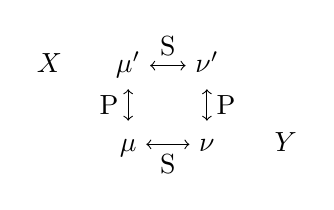
\begin{tikzpicture}

\snode{X}{-1,0}{X};

\snode{MUP}{0,0}{\mu'};
\snode{MU}{0,-1}{\mu};

\snode{NUP}{1,0}{\nu'};
\snode{NU}{1,-1}{\nu};

\snode{Y}{2,-1}{Y};

\draw[<->] (MUP) -- (MU) node [midway, left] () {P};
\draw[<->] (NUP) -- (NU) node [midway, right] () {P};
\draw[<->] (MU) -- (NU) node [midway, below] () {S};
\draw[<->] (MUP) -- (NUP) node [midway, above] () {S};

\end{tikzpicture}
\end{center}
\noindent which suggests that the AO-DF-SOS-MP2 has an overall asymptotic scaling of $\ccpx{3}$. With local density fitting, the graph can however become fully connected
\begin{center}
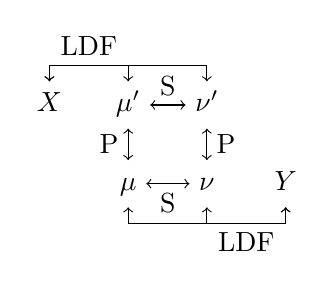
\begin{tikzpicture}

\snode{X}{-1,0}{X};

\snode{MUP}{0,0}{\mu'};
\snode{MU}{0,-1}{\mu};

\snode{NUP}{1,0}{\nu'};
\snode{NU}{1,-1}{\nu};

\snode{Y}{2,-1}{Y};

\draw[<->] (MUP) -- (MU) node [midway, left] () {P};
\draw[<->] (NUP) -- (NU) node [midway, right] () {P};
\draw[<->] (MU) -- (NU) node [midway, below] () {S};
\draw[<->] (MUP) -- (NUP) node [midway, above] () {S};

\draw[<->] (X.north) |- (-0.5,0.5) node[above] {LDF} -| (MUP.north);
\draw[<->] (X.north) |- (-0.5,0.5) node[above] {} -| (NUP.north);

\draw[<->] (Y.south) |- (1.5,-1.5) node[below] {LDF} -| (MU.south);
\draw[<->] (Y.south) |- (1.5,-1.5) node[below] {} -| (NU.south);

\end{tikzpicture}
\end{center}

\noindent where "LDF" is the sparsity relationship introduced between the auxiliary density $X$ and the product density $\cbra{\mu\nu}$, which is metric-specific. In the case of quasi-robust density fitting, LDF = S, and the intermediates $\mathbf{Z}\pa$ can be constructed with linear effort. For weaker decay behaviour, such as the error function coulomb-attenuated metric, the scaling is intermediate between linear and quadratic (Gla2020). 

% Mau2014 https://aip.scitation.org/doi/full/10.1063/1.4881144
% Gla2020 https://pubs.acs.org/doi/abs/10.1021/acs.jctc.0c00600

% QQR screeening:
% S. A. Maurer, D. S. Lambrecht, D. Flaig, and C. Ochsenfeld, J. Chem. Phys. 136, 144107 (2012). https://doi.org/10.1063/1.3693908
%  S. A. Maurer, D. S. Lambrecht, J. Kussmann, and C. Ochsenfeld, J. Chem. Phys. 138, 014101 (2013). https://doi.org/10.1063/1.4770502

\subsection{SVO-MP2 flavours}

Among the eraliest

Use a different approach than Laplace: Hylleraas Functional

Sparsity relation ship [ij] <-> [ab]

\subsection{NTO-MP2 ?}

% Hylleraas functional: 
% Hyl1930 https://link.springer.com/article/10.1007/BF01397032

% First use of LMO+PNOs with Hylleraas 
% Pul1986 https://link.springer.com/article/10.1007%2FBF00526697

% LInear scaling of the functional
% Linear scaling of electron inetgrals
% linear scaling of MO-AO transformation -> or density fitting

\section{Low-Scaling Correlated Excited State Methods}
Local CC2, PNO-ADC, Mester-ADC, Mester-CC2, NTO-CC2, CornFlex

% PAO CCLR not good! Look at Gunnar review article perhaps

\subsection{CC2}


\subsection{ADC}



\part{Benchmarking: Timings and }

OTHER: \url{https://www.kth.se/blogs/pdc/2018/11/scalability-strong-and-weak-scaling/}

\part{Annex}

- ERI deomposition: cholesky, THC, pseudo-spectral
% cholesky https://link.springer.com/article/10.1007/s00214-009-0608-y
- The evil matrix inversion: considerations
% see https://www.johndcook.com/blog/2010/01/19/dont-invert-that-matrix/ 
% also https://epubs.siam.org/doi/abs/10.1137/1.9780898718027.ch14

\end{document}